\centering
\subfigure[Network structure.]{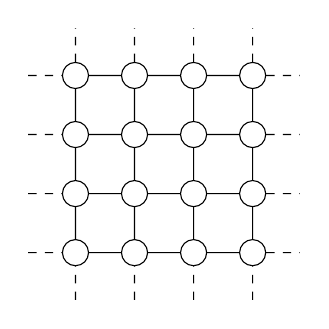
\begin{tikzpicture}
  [every node/.style={shape=circle,minimum size=0.1cm,draw},scale=0.75]
\foreach \x in {1,2,3,4} \foreach \y in {1,2,3,4}
   \node (\x\y) at (\x,\y) {};
\foreach \x in {1,2,3,4} {
  \coordinate (\x0) at (\x,0.2) {} ;
  \coordinate (\x5) at (\x,4.8) {} ;
}
\foreach \y in {1,2,3,4} {
  \coordinate (0\y) at (0.2,\y) {} ;
  \coordinate (5\y) at (4.8,\y) {} ;
}
\draw
  \foreach \x in {1,2,3,4}
    \foreach \ya/\yb in {1/2,2/3,3/4}
      { (\x\ya) -- (\x\yb) }
  \foreach \y in {1,2,3,4}
    \foreach \xa/\xb in {1/2,2/3,3/4}
      { (\xa\y) -- (\xb\y) }
;
\draw[dashed]
  \foreach \x in {1,2,3,4}
    { (\x0) -- (\x1) (\x4) -- (\x5) }
  \foreach \y in {1,2,3,4}
    { (0\y) -- (1\y) (4\y) -- (5\y) }
;
\end{tikzpicture}}%
\hspace{0.5cm}%
\subfigure[Message routing in an intact network.]{\label{f:mesh:route}%
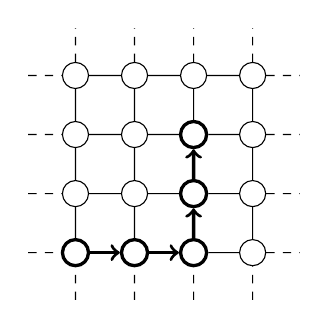
\begin{tikzpicture}
  [every node/.style={shape=circle,minimum size=0.1cm,draw},scale=0.75]
\node [very thick] (11) at (1,1) {};
\node [very thick] (21) at (2,1) {};
\node [very thick] (31) at (3,1) {};
\node []      (41) at (4,1) {};
\node []      (12) at (1,2) {};
\node []      (22) at (2,2) {};
\node [very thick] (32) at (3,2) {};
\node []      (42) at (4,2) {};
\node []      (13) at (1,3) {};
\node []      (23) at (2,3) {};
\node [very thick] (33) at (3,3) {};
\node []      (43) at (4,3) {};
\node []      (14) at (1,4) {};
\node []      (24) at (2,4) {};
\node []      (34) at (3,4) {};
\node []      (44) at (4,4) {};

\draw [very thick,->] (11) -- (21) ;
\draw [very thick,->] (21) -- (31) ;
\draw                                      (31) -- (41)
                 (12) -- (22) (22) -- (32) (32) -- (42)
                 (13) -- (23) (23) -- (33) (33) -- (43)
                 (14) -- (24) (24) -- (34) (34) -- (44) ;

\draw [very thick,->] (31) -- (32) ;
\draw [very thick,->] (32) -- (33) ;
\draw                                      (33) -- (34)
                 (11) -- (12) (12) -- (13) (13) -- (14)
                 (21) -- (22) (22) -- (23) (23) -- (24)
                 (41) -- (42) (42) -- (43) (43) -- (44) ;

\foreach \x in {1,2,3,4} {
  \coordinate (\x0) at (\x,0.2) {} ;
  \coordinate (\x5) at (\x,4.8) {} ;
}
\foreach \y in {1,2,3,4} {
  \coordinate (0\y) at (0.2,\y) {} ;
  \coordinate (5\y) at (4.8,\y) {} ;
}
\draw[dashed]
  \foreach \x in {1,2,3,4}
    { (\x0) -- (\x1) (\x4) -- (\x5) }
  \foreach \y in {1,2,3,4}
    { (0\y) -- (1\y) (4\y) -- (5\y) }
;
\end{tikzpicture}}%
\hspace{0.5cm}%
\subfigure[Node failure requires use of an alternate route.]{%
\label{f:mesh:fail}%
\begin{tikzpicture}
  [every node/.style={shape=circle,minimum size=0.1cm,draw},scale=0.75]
\node [very thick] (11) at (1,1) {};
\node [very thick,fill=gray] (21) at (2,1) {};
\node []      (31) at (3,1) {};
\node []      (41) at (4,1) {};
\node []      (12) at (1,2) {};
\node [very thick] (22) at (2,2) {};
\node [shape=starburst,starburst points=9,
       starburst point height=.3cm,random starburst=1434]
                   (32) at (3,2) {};
\node []      (42) at (4,2) {};
\node []      (13) at (1,3) {};
\node [very thick]      (23) at (2,3) {};
\node [very thick] (33) at (3,3) {};
\node []      (43) at (4,3) {};
\node []      (14) at (1,4) {};
\node []      (24) at (2,4) {};
\node []      (34) at (3,4) {};
\node []      (44) at (4,4) {};

\draw [very thick,->] (11) -- (21) ;
\draw [very thick,->] (23) -- (33) ;
\draw                         (21) -- (31) (31) -- (41)
                 (12) -- (22)
                 (13) -- (23)              (33) -- (43)
                 (14) -- (24) (24) -- (34) (34) -- (44) ;

\draw [very thick,->] (21) -- (22) ;
\draw [very thick,->] (22) -- (23) ;

\draw                                      (33) -- (34)
                 (11) -- (12) (12) -- (13) (13) -- (14)
                                           (23) -- (24)
                 (41) -- (42) (42) -- (43) (43) -- (44) ;

\foreach \x in {1,2,3,4} {
  \coordinate (\x0) at (\x,0.2) {} ;
  \coordinate (\x5) at (\x,4.8) {} ;
}
\foreach \y in {1,2,3,4} {
  \coordinate (0\y) at (0.2,\y) {} ;
  \coordinate (5\y) at (4.8,\y) {} ;
}
\draw[dashed]
  \foreach \x in {1,2,3,4}
    { (\x0) -- (\x1) (\x4) -- (\x5) }
  \foreach \y in {1,2,3,4}
    { (0\y) -- (1\y) (4\y) -- (5\y) }
;
\end{tikzpicture}}%
\caption{Idealized mesh network.}%
